% !TeX root = ../main.tex

\chapter{编译器中端优化}
\section{中端优化处理简介}
\subsection{Pass简介}

顾名思义,Pass就是“遍历一遍IR”的意思。在本项目的设计和实现中,基于类Pass的派生类有两个,它们的名称和功能如下:

1. Analysis,只遍历和分析IR,不对IR进行转换,用于得出一些结论,方便后续变换,如支配树分析,活跃变量分析等。

2. Transform,遍历和转换IR,根据一些优化算法对IR做优化,如控制流图简化,循环不变量外提,死代码消除等。

所有的Pass类都要重写虚函数run,用于表示这个Pass应该对IR做哪些分析或者变换,编译器需要哪些Pass,就将其添加到一个列表中,再统一检查和执行,这种设计可以降低编译器的耦合性,方便了编译器的拓展和裁剪。后文介绍每个Pass时,都会对其run方法着重介绍。

\subsection{本项目对Pass的管理}

具体项目实现上,编译器设计了一个管理Pass对象的类PassManager。

\begin{figure}[htb]
  \centering
  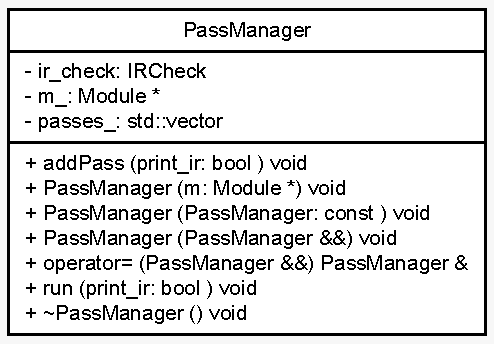
\includegraphics[width=0.6\textwidth]{figures/PassManagerUML.pdf}
  \caption{PassManager类成员变量和函数示意图}
  \label{fig:passMnager}
\end{figure}

图中的数据结构和成员函数的解释说明如下:

1. ir\_check 是函数指针,指向IR合法性检查的函数对象

2. m\_是Module类指针,是对要处理的编译文件的IR数据结构

3.passes\_是一个向量对象,存储要进行的Pass,通过addPass方法向其增加需要的Pass。

PassManager的run方法会顺序检查和调用passes\_中的所有优化,具体的控制流程图如下:
 
\begin{figure}[htb]
  \centering
  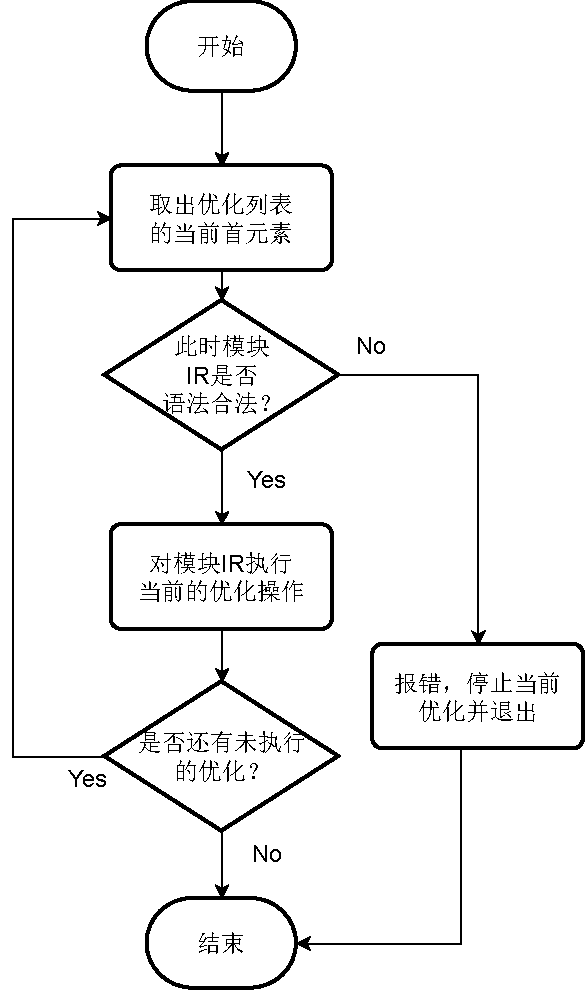
\includegraphics[width=0.7\textwidth]{figures/passManagerRunMethod.pdf}
  \caption{编译器使用PassManager管理每个IR Pass的流程图}
  \label{fig:passMnagerRun}
\end{figure}

\section{控制流程图简化}
\subsection{控制流程图的定义}
控制流程图(control-flow graph)简称CFG,是编译器静态分析和代码优化的核心技术与重要环节。

上一章定义了基本块,即满足只能从入口指令进入该基本块,只能从末尾指令离开该基本块两个条件的指令序列。控制流程图的是结点即为基本块。

而控制流程图中的边对应了基本块之间的跳转关系,例如,基本块B1到基本块B2之间有一条边当且仅当B1的末尾有跳转到B2的分支指令,此时称B1为B2的前驱,同样地,称B2为B1的后继。

在一个基本块内部,平均是4到6条指令,它们往往彼此数据相关,完成对变量的操作如逻辑判断或算术运算等;同时基本块通过彼此之前跳转的逻辑关系,可以实现循环,条件分支等程序控制逻辑,进而组成函数,可以认为控制流程图是整个IR从源代码到实际指令承上启下的表示。

因此,对基本块构成的控制流程图的简化会直接通过影响函数执行基本块的数量来影响编译结果性能的好坏。

\subsection{简化控制流程图算法}

控制流程图简化的主要目的是消除不可达或者冗余的基本块:

1. 若其他Pass生成了某个无前驱的基本块,那么该基本块即为不可达基本块,可以将其删除

2. 若某个基本块仅可从其前驱跳转过来,且其前驱也只能跳转到该基本块,那么这条跳转语句显然是多余的,可以将该基本块和前驱合并

具体而言,该优化Pass会对IR中的所有函数顺序执行一些优化,首先是处理上一个Pass产生的冗余流程图:

1.  RemoveNoPredecessorBB: 如果某basic block不是entryBB且无前驱,说明控制流不会到达该基本块,标记该bb为待删除,对其后继的所有succbb,在它们的前驱列表中移除bb;对于后继bb的所有指令,如果是$\phi$指令,因为这条指令少了个待选择的基本块,修改这些$\phi$指令的参数。

2. EliminateSinglePredecessorPhi: 如果某个$\phi$指令($\phi$指令将在下文介绍,这里只需直到$\phi$指令define的对象和$\phi$指令的参数列表有关)的参数仅有一个,则这个$\phi$指令可能的值就确定为那个唯一的参数,将该$\phi$指令的use对象替换为$\phi$指令的参数。

3. MergeSinglePredecessorBB: 对每个基本块,如果其仅有一个前驱基本块prebb,若prebb的最后一条指令br满足仅有一个跳转分支,可以删除br,把bb的指令挪到bb的前驱中,更新bb后继的前驱,更新对bb的所有使用为指向prebb,完成前前驱基本块和其前驱的合并。

然后处理可能由以上转换导致的无效流程图节点:

4. RemoveSelfLoop: 如果前驱基本块仅有一个而且这个前驱基本块就是自身,标记为删除。selfloop不会直接出现在IR builder的结果中,只会由其他IR转换导致。

5. RemoveNoPredecessorBB: 如果某个基本块不可达,即从入口基本块无法访问,将其标记为删除。同样的,NoPredecessorBB不会直接出现在IR builder的结果中,只会由其他IR转换导致。


该Pass的run方法伪代码描述如~\ref{algo:simplifyCFG}。

\begin{algorithm}[htb]
  \small
  \SetAlgoLined
  \KwData{IR of a compiler module}
  \KwResult{module with simplified CFG}

  \For{func in module.getFuns()}{
    RemoveNoPredecessorBB()\;
    EliminateSinglePredecessorPhi()\;
    MergeSinglePredecessorBB()\;
    EliminateSingleUnCondBrBB()\;

    RemoveSelfLoopBB()\;
    RemoveNoPredecessorBB()\;

    EliminateSinglePredecessorPhi()\;
  }
  \caption{SimplifyCFG Pass Run Method}
  \label{algo:simplifyCFG}
\end{algorithm}

run方法内首先尝试对上个Pass产生的冗余控制流进行消除,这说明该Pass不应该直接用于刚刚经过前端分析而生成的IR,否则如上所述该优化Pass只能消除一些空函数或者无条件跳转等冗余节点。但是在后续的各种优化和变形中,程序的IR形式很可能会发生改变,甚至产生包含冗余或者根本不可达的无效控制流。

因此,我们可以得出该Pass在整个PassManager中的passes列表中应该是多次出现的,具体而言,如果执行了Transform类的Pass,那么应该在后续安排一次控制流程图的简化。

例如,经过死代码删除,这个基本块只剩下了跳转指令,那么可以删掉这些跳转指令,把该基本块的前驱的跳转目标地址设置为该基本块的后继基本块;再例如,经过常量传播,某些条件分支指令的条件被计算出了逻辑真假,而程序又不可能跳转到逻辑为假的分支目标基本块,就也可以删掉这个无用的基本块;更为常见的,一旦修改了某个基本块的分支语句,就必须检查该基本块的后继中的$\phi$指令(将在第三节介绍)参数列表。

以上就是控制流程图简化算法对其他IR Pass优化的重要作用,值得一提的是,在本项目的Main方法中的45个Pass中,控制流程图简化和死代码消除就占据了21个。


\subsection{应用举例}

为了说明优化Pass对代码执行效率的重要作用,这里以比赛中的测试用例if.sy为例子说明,该测试用例的代码如下:

\begin{verbatim}
    int main() {
      int a;
      a = 5;
      int b;
      b = 10;
      if(a == 5)
        if (b == 10) 
          a = 25;
        else 
          a = a + 15;
      return a;
    }
\end{verbatim}

由源代码,可以看出,该函数能够通过编译时静态分析得到执行结果25,直接翻译得到IR,并把IR按照各个基本块的跳转关系组织,得到CFG,在中端为了满足静态单赋值的要求, 各个基本块中使用变量都需要 Load 和 Store 操作,造成大量冗余,所以我们首先将其转换成 Reg-SSA 形式,用虚拟寄存器来引用变量,可以减少LS次数,得到如图的IR,这些虚拟寄存器在后端时用图染色算法再对应到到物理寄存器。


此时得到的控制流程图如图~\ref{fig:cfg0}。




\begin{figure}[htb]
  \centering
  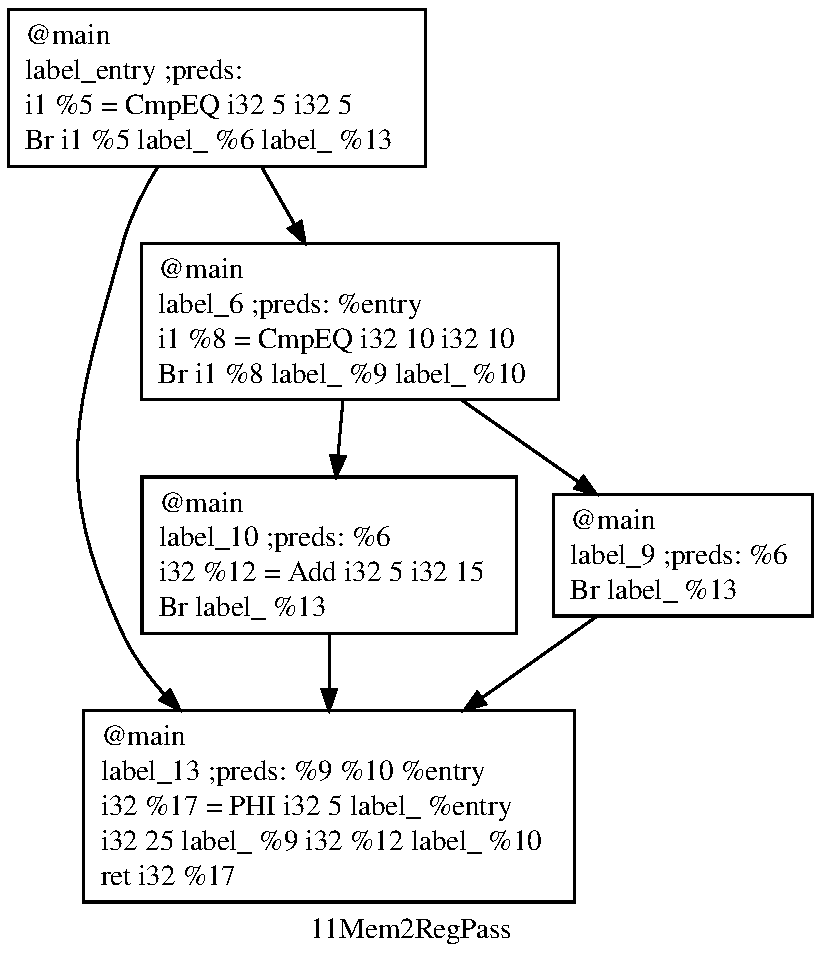
\includegraphics[width=0.7\textwidth]{figures/cfgsimplify0.pdf}
  \caption{简化控制流之前}
  \label{fig:cfg0}
\end{figure}

继续观察可以发现,有些基本块末尾的比较和分支指令,能够在编译时就得到结果,如图中对常量5和5进行的Cmp指令,经过常量传播Pass之后,就可以确定分支跳转的目标,最后经过控制流图简化,消除冗余的单目标分支指令,就得到了最终的结果 25。

\begin{figure}[htb]
  \centering
  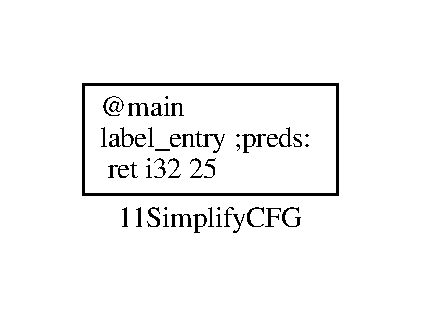
\includegraphics[width=0.4\textwidth]{figures/cfgsimplify1.pdf}
  \caption{简化控制流之后}
  \label{fig:cfg1}
\end{figure}
